\documentclass[../../main.tex]{subfiles}
\begin{document}
\subsection{Software Lösungskonzepte}
Die Steuerungssoftware, welche auf dem Hauptrechner ausgeführt wird, soll in mehrere Teilprogramme aufgeteilt werden.
Teilprogramme können so unabhängig voneinander implementiert und getestet werden.
Um anschliessend zwischen den Teilprogrammen zu kommunizieren, wird eine Middleware verwendet. Die Middleware kann auch genutzt werden,
um die einzelnen Teilprogramme zu testen. Zusätzlich können verschiedene Programmiersprachen für die einzelnen Teilprogramme verwendet werden.
Dies erhöht zusätzlich die Flexibilität während der Entwicklung.

\subsubsection{Architektur}
Im folgenden Diagramm wird die Architektur der Steuerungssoftware aufgezeigt
\begin{figure}[H] %Architektur mit Middleware
    \centering
    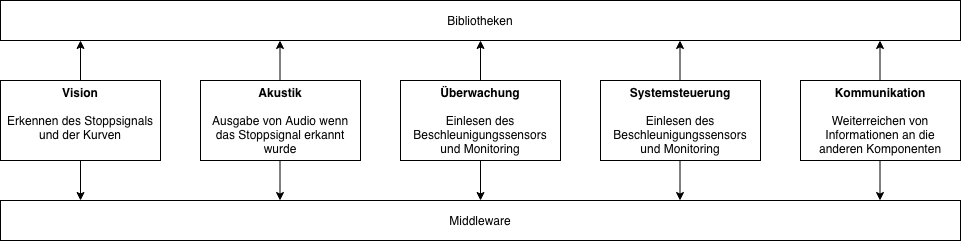
\includegraphics[width=1.0\textwidth]{drawings/ArchitekturDiagramm/SW_Architektur_Middleware.png}
    \caption {Software Architektur Middleware. Gezeichnet mit https://draw.io}
\end{figure}

\textbf{Legende:}
\begin{itemize}
    \item Die Pfeile visualisieren die Abhängigkeiten innerhalb der Architektur
\end{itemize}

\subsubsection{Technologie}
Während der Technologierecherche wurde eine Analyse gemacht, um zu entscheiden welche Technologie eingesetzt werden soll. Bald wurde ZeroMQ
auserkoren, da diese schlank ist und ohne Performance Probleme auf kleinen Einplatinenrechner läuft. Ausserdem ist die Middleware bekannt
und hat eine hervorragende Dokumentation. Um die Daten, welche über die Middleware geschickt werden, mit verschiedenen Programmiersprachen zu
nutzen, wird Protobuffers verwendet. Protobuffers ist ein Format zur Berschreibung von Daten. Dieses Format kann anschliessend verwendet werden, um
Klassen bzw. Funktionen für fast jede Programmiersprache zu benutzen. Das heisst, dass die Daten einmalig definiert werden und anschliessend von
allen Teilprogrammen verwendet werden können.

\textbf{Beispiel Protobuf:}
\lstinputlisting{../src/raspi/pb/direction.proto}
Man sieht nun, dass eine 'Direction' Mitteilung definiert wird. Diese hat ein String Attribut, welches direction heisst. Mit dieser Definition
wird mithilfe eines 'protobuffer compiler' Code generiert. Dieser kann die definierte Message Serialisieren und Deserialisieren.

\textbf{Beispiel Generierung für Python:}
\begin{lstlisting}
    protoc -I=pb --python_out=pb pb/direction.proto
\end{lstlisting}
Mithilfe von diesem Beispiel wird die Protobuf Definition (direction.proto) zu Python Code generiert.

\textbf{Beispiel Generierter Python Code:}
\lstinputlisting[language=Python]{../src/raspi/pb/direction_pb2.py}
Das generierte Python File, welches mithilfe des 'protobuffer compiler' erzeugt wurde.

\subsubsection{Proof-of-Concept}
Um zu testen, ob eine Kommunikation zwischen zwei Prozessen mithilfe der Middleware möglich ist, wurde eine kleine Testsoftware entwickelt.
Dabei wurde das 'direction.proto' File verwendet, um von einem Prozess eine Richtung (Direction) zu einem anderen
Prozess zu senden und zu empfangen.

\subsubsection{Performance}
Die Performance wurde nicht gemessen und verifiziert. Jedoch wurden bei den Tests keine Limitationen gefunden. Deshalb kann davon ausgegangen werden,
dass die Performance für unseren Anwendungsfall ausreicht. Ausserdem werden nur wichtige Events zwischen den Prozessen ausgetauscht und somit ist die Datenrate
eher zweitrangig. Die Latenz ist jedoch sehr zentral um einen möglichst agilen Regelkreis zu implementieren. Hier bewegt sich ZeroMQ zwischen 450us - 700us.

\textbf{Performance Tests:}
\begin{itemize}
    \item http://zeromq.org/area:results
    \item http://nikolaveber.blogspot.com/2011/04/if-you-are-planning-large-or-not-even.html
\end{itemize}

\end{document}
